\section{Introduction}
\label{sec:intro}

Online multi-object tracking (MOT)~\cite{wojke2017simple,feichtenhofer2017detect,bergmann2019tracking,zhang2020fair} aims at localizing a set of objects (\eg, pedestrians), while following their trajectories over time so that the same object bears the same identities in the entire input video stream. 
Earlier methods mostly solved this problem with two separate stages:
1) the object detection stage that detects object instances in individual frames~\cite{felzenszwalb2009object,ren2015faster,liu2016ssd,zhou2019objects,ge2021yolox}; and 2) the data association stage that links the detected object instances across time~\cite{braso2020learning,zhang2020fair} by modeling the state changes of tracked objects and solving a matching problem between them and the detection results.
Though recent studies~\cite{meinhardt2021trackformer,zeng2021motr} suggest that combining these two stages could be beneficial, the combination usually leads to the undesired simplification of the association module in modeling the change of the objects in time.  

% It requires not only accurate object detection in individual video frames, but also robust association~\cite{braso2020learning,zhang2020fair} to link objects using their ever-changing appearances and positions.
In this paper, we propose a Transformer-based tracking model, called \emph{MeMOT}, that performs object detection and association under a common framework in an online manner. 
The key design of MeMOT is to build a large spatio-temporal memory that stores the past observations of the tracked objects. The memory is actively encoded in every time step by referencing relevant information so that the states of the objects are more accurately approximated for the association task.
The rich representation of the tracked objects extracted from the spatial-temporal memory enables us to solve the object detection and association tasks in a unified decoding module. It directly outputs object instances that have been tracked and reappears in the latest frame and novel object instances that are first time seen.
The idea of MeMOT is illustrated in Fig.~\ref{fig:teaser}. 

\begin{figure}
    \centering
    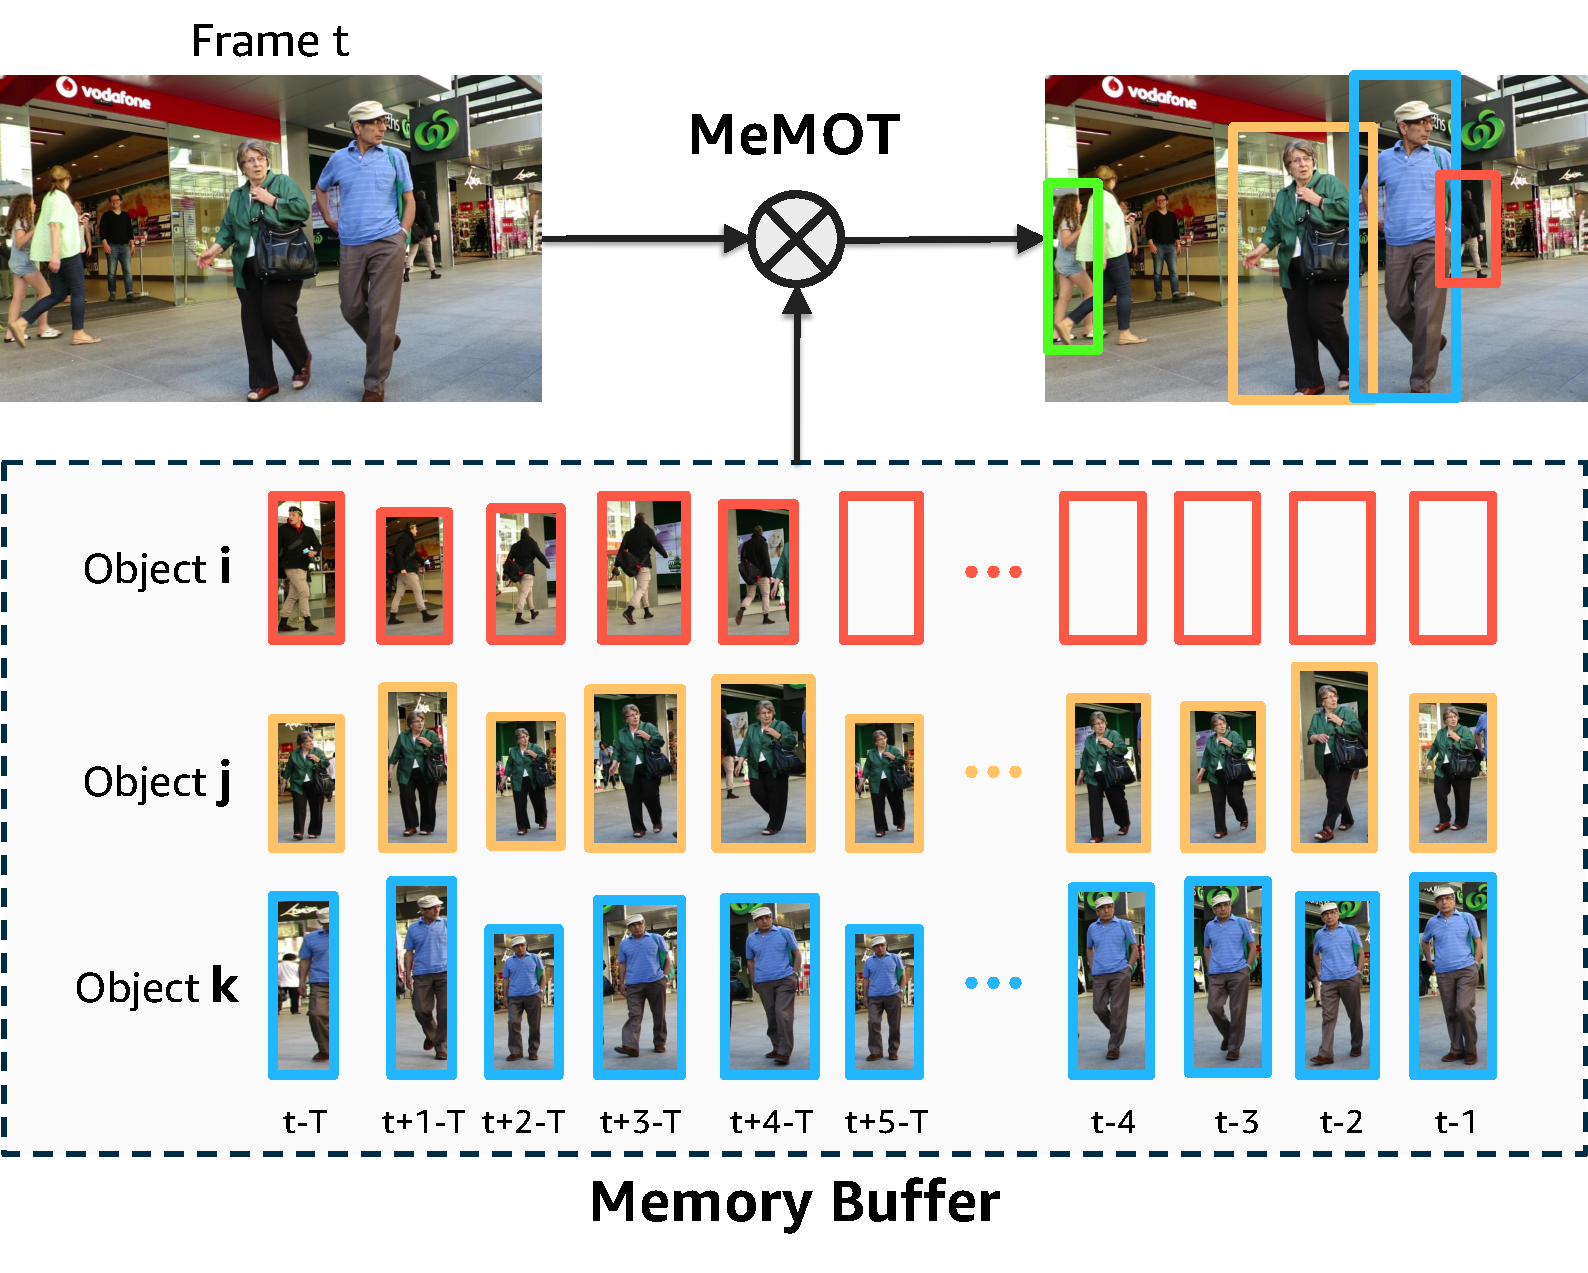
\includegraphics[width=0.97\linewidth]{figures/teaser.pdf}  
    \vspace{-4.5mm}
    \caption{\textbf{Illustration of the idea of MeMOT}.
    A spatio-temporal memory stores a long range states of all tracked objects and is updated over time.
    Each row in the memory buffer represents an active tracklet.
    The ``person crops'' indicate that their the history states are preserved in the memory, and the blank box indicates this person does not appear in the frame at that time, occluded or not detected.
    The tracking plots show that MeMOT can maintain active tracks (yellow and blue boxes), link reappearing tracks after occlusion (red box), and generate new objects (green box).}
    \vspace{-2.5mm}
    \label{fig:teaser}
\end{figure}

At each time step, MeMOT runs the following three main components:
1) a \textit{hypothesis generation} module that produces object proposals from input image feature maps as a set of embedding vectors;
2) a \textit{memory encoding} module that encodes the spatial-temporal memory corresponding to each tracked object into a vector known as the track embedding;
and 3) a \textit{memory decoding} that inputs the proposal and track embeddings and solves the object detection and data association tasks simultaneously for multi-object tracking.
The hypothesis generation module is implemented by a Transformer-based encoder-decoder network~\cite{carion2020end,zhu2020deformable}.
It produces a set of embedding vectors, known as the \emph{proposal embedding}, each representing one hypothetical object instance. 
The memory encoding module first divides the spatial temporal memory on each object into short- and long-term memories and aggregates them each into one embedding vector through cross attention modules~\cite{vaswani2017attention}. The two vectors then interact through the self-attention mechanism to produce the \emph{track embedding} of the tracked object at this time step. 
The proposal and track embeddings, together with the original image features, are then fed to the memory decoding module.
For each track embedding, it produces the location and the visibility of the object being tracked in this frame. For each proposal embedding, it predicts whether this hypothetical object instance is depicting a novel object, a tracked object, or simply a background region. 
An illustration of the MeMOT model is shown in Fig.~\ref{fig:network}.
The entire model can be trained end to end on video datasets with object bounding box and identity annotations.
During inference, we obtain the tracking outputs in one inference run of the model at each time step, \emph{without} any extra optimization~\cite{rangesh2021trackmpnn, chu2021transmot} or post-processing~\cite{sun2020transtrack, bergmann2019tracking, zhang2020fair}. 

We evaluate MeMOT on the MOT Challenge~\cite{milan2016mot16,dendorfer2020mot20} benchmarks for pedestrian tracking.
Experimental results show that MeMOT achieves the state-of-the-art performance among all algorithms with an in-network association solver and is competitive with those utilizing a post-network association process.
Specifically, MeMOT outperforms other Transformer-based methods in both object detection and data association.
Extensive ablation studies further validate the design and effectiveness of MeMOT.
